\documentclass{article}

\usepackage[dutch]{babel}
\usepackage{graphicx}
\usepackage{hyperref}
\usepackage{marvosym}
\usepackage{url}

\begin{document}

\title{Inrichting Centrale Bank}
\author{Paul Wondel}
\date{\today}
\maketitle

\begin{abstract}
In opdracht voor project 4 heb ik dit verslag opgesteld.
In dit verslag worden er de kwaliteitseisen en functionaliteitseisen
beschreven voor de inrichting van de Centrale Bank.
De vraag die gesteld wordt is: "Hoe richt ik efficient een centrale bank op?".
In dit verslag wordt er antwoord gegeven op deze vraag.
\end{abstract}

\clearpage
\newpage

\tableofcontents

\clearpage
\newpage

\section{Analyse: Inrichting Centrale Bank}
\vspace{6mm}
\subsection{Server Communicatie}
\begin{figure}[h]
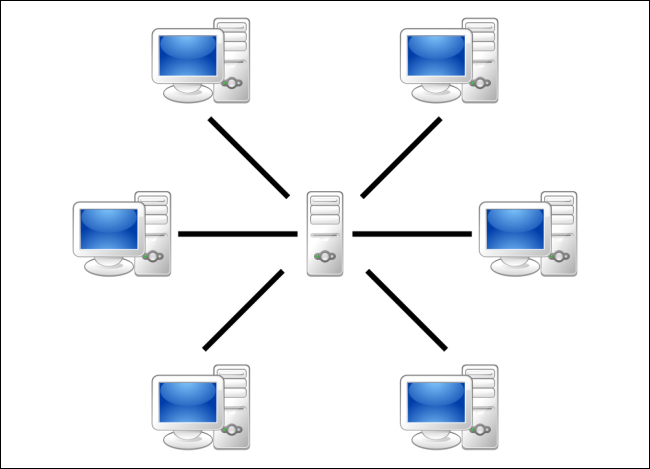
\includegraphics[height=6cm, width=8cm]{centralserver.png}
\centering
\end{figure}

\paragraph{Centrale Server}
De Centrale Bank zal fungeren als een zogenaamd tussenpersoon.
De Centrale Bank is verbonden met alle lokale banken.
Als een lokale bank data nodig heeft van een andere lokale bank,
kan hij de gegevens opvragen door een aanvraag naar de centrale bank te sturen.
De centrale bank vervolgens stuurt de aanvraag naar de geadresseerde lokale bank.
Die stuurt, op zijn beurt, de gegevens naar de centrale bank waardoor de centrale bank
de gegevens terug kan sturen de lokale bank die de gegevens had aangevraagd.
Het sturen van data duurt wel iets langer dan peer to peer netwerken,
maar het verwerken van de data is veel efficienter bij de lokale banken.
Dit vanwege het feit dat het meeste werk belast valt bij de centrale server.
Bij het gebruikerseinde is dit veel fijner om te zien,
want dan zijn de ATMs niet te langzaam bij het tonen van informatie.

Deze gang van zaken vindt plaats d.m.v. servers.
Elke lokale bank heeft een database waarin alle gegevens van hun klanten in staan.
Deze databases staan op een server van de lokale bank (dus een lokale server).
De servers van de lokale banken zullen verbonden zijn aan een centrale server
van de centrale bank.
De databases zijn SQL-type databases.
Om data uit de databases te halen moeten er query commandos verstuurd worden.
Door middel van Message queuing of MQTT kunnen er een aantal queries tegelijk verstuurd worden.
De connectie tussen de lokale server en de centrale server moeten wel beveiligd zijn.
Hiervoor kunnen er protocollen toegepast worden, namelijk TLS (nu SSL).
SSL zorgt ervoor dat de data die verstuurd wordt over deze connectie beveiligd is
d.m.v. encryptie.
De encryptie maakt de data onleesbaar voor externe afluisteraars.
Door het gebruik van een centrale server is er geen probleem in welke
programmeer taal de clients van de lokale banken geschreven zijn.
De applicatie die draait op de centrale server vertaald de quaries
die de lokale banken sturen en stelt dan zijn eigen query op voor
waarmee hij dan een aanvraag aan maakt.
Dit wordt dan gedaan d.m.v. certificaten. 

Mocht er een nieuwe lokale bank ontstaan die wenst mee te doen aan dit systeem,
dan is het helemaal niet moeilijk om hem aan te sluiten aan het netwerk.
Zijn programmeertaal is niet van belang omdat de server alle talen aankan.
Ook is het makkelijker omdat de nieuwe lokale bank alleen verbonden
hoeft te zijn aan de centrale server.
Via de centrale server kan hij in contact komen met de andere lokale banken.

\vspace{5mm}

\begin{figure}[h]
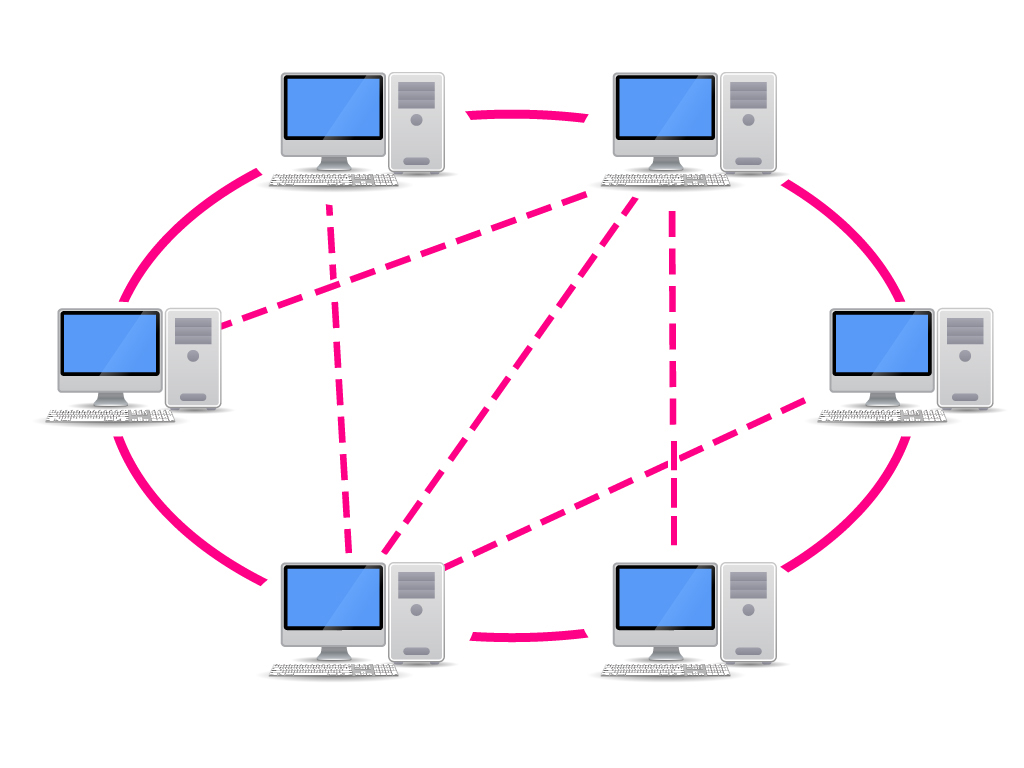
\includegraphics[height=6cm, width=8cm]{peertopeer.jpg}
\centering
\end{figure}

\paragraph{Peer-to-Peer Netwerk}
Een peer to peer netwerk is een netwerk waarbij verschillende servers met
elkaar verbonden zijn.
In het figuur hierboven is een schets van het netwerk model gemaakt.
In dit model zijn alle lokale banken met elkaar verbonden.
Als een lokale bank data nodig heeft van een andere bank,
dan stuurt hij een aanvraag rechtstreeks naar de lokale bank
waarvan hij data nodig heeft.
De andere lokale bank stuurt dat gewoon de data naar de lokale bank
die de aanvraag verstuurd heeft.
Met het peer to peer netwerk gaat het versturen van data veel sneller
dan data versturen via een centrale server.

In dit model horen alle lokale banken wel in dezelfde programmeertaal geschreven te worden.
Dit is om te voorkomen dat de aanvragen die verstuurd worden onleesbaar zijn.
Dus het versturen van data gaat vrij snel omdat er geen vertaling plaats hoeft te vinden
Het verwerken van data is ook langzamer aan het gebruikerseinde dan bij
het gebruik van een centrale server.
De lokale banken zijn verbonden met alle lokale banken in de regio.
Dit brengt veel werk belast met zich mee.
Omdat de banken een constante connectie moeten openhouden met elkaar.
Hiervoor moeten er veel resources gebruikt worden om dit stand te houden.
Hiernaast hoort hij constant data te verwerken om aan de eindgebruiker te tonen.
Al dit werkbelast maakt het gebruik bij de ATM niet prettig voor de klant.
De klant zal langer moeten wachten om de gegevens tevoorschijnt te krijgen.

Bij deze connectie hoort er ook encryptie te zijn.
De encryptie zal hier helaas per connectie moeten geschieden.
Als er bijvoorbeeld 50 banken in de regio zijn,
zal elke bank 49 connecties open hebben staan.
Alle 49 connecties horen dan ook met ge-encrypt te zijn met b.v. SSL/TLS.
Dit neemt dan ook veel resources van de bank.

\subsection{Certificaten}
Certificaten gebruiken bij het aanvragen van data is een goede manier
om data te versturen tussen verschillende clients in verschillende programmeertalen.
Een certificaat is data opsturen in een bepaald formaat om bepaald data uit het
database te krijgen.
De centrale server vertaald dit certificaat in SQL queries en stuurt die dan naar
de databases.
De databases sturen dan de data op naar de centrale bank.
De centrale bank stuurt dan de data weer in een certificaat formaat
zodat de lokale bank de gegevens kan lezen.
Het cerficiaat kan b.v. bestaan uit een bankpasnummer en een pincode.
Bij het inloggen bij een bank wordt de cerficitaat opgestuurd naar de centrale bank.
Na het verwerken van de data met het database,
geeft de centrale bank een response.
Aan de hand van het response kan de lokale bank verder gaan met het
verwerken van de data die hij ontvangen heeft.

De certificalen worden op de centrale server gemaakt en vertaald door een applicatie.
Deze applicatie is in Java geschreven.
Deze applicatie vertaald de certificaten in SQL queries en stuurt de data,
verkregen het database, terug naar de lokale banken.
De banken moet er voor zorgen dat er in hun eigensysteem het sturen en
verwerken van certificaten mogelijk is.

\subsection{Message Protocols}

\subsubsection{MQ: Message Queuing}
Berichten worden door verschillende programmas gebruikt
om data met elkaar te delen tussen een zender en ontvanger.
Programmas gebruiken veel berichten na elkaar maar niet
alle berichtn kunnen tegelijk verwerkt worden.
Daarom is er een queue. Een gueue is een lijst met wachtende onderwerpen.
Message Queuing zorgt ervoor dat de messages in een volgorde verstuurd worden.

Message Queuing is een asynchroon communicatie protocol.
Dat houdt in dat het systeem een bericht in een queue lijst plaatst
en dat hoeft niet per direct verwerkt te worden.
Email is een voorbeeld van asynchroon communicatie.

Bij message queuing wordt er gebruik gemaakt van decoupling.
Dit is om de afzender en ontvanger te van elkaar te scheiden.
Decoupling is een proces dat delen van een systeem die afhankelijk
zijn van elkaar scheidt en zelfstandig maakt.

Message queuing werkt als volgt.
Een message producer(een applicatie bv) maakt een message aan met data erin.
De message stuurt hij dan naar een 'Message Broker'.
Een Message Broker houdt de message queue bij.
Wanneer de producer al zijn messages naar de message broker
gestuurd heeft stuurt de message broker de message queue naar
de message consumer.
De message consumer kan nu een voor een de messages in de message queue
verwerken en hoeft zo niet alle messages tegelijk te behandelen.
De messages hebben allemaal een topic.
Aan de hand van de topic reageren de message clients op de message queue die
door de message broker verstuurd wordt.


MQ brengt vele voordelen met zicht mee.
MQ heeft redundantie via persistentie om data te blijven behouden.
Je kan batches met messages zodat niet elke message appart wordt
verstuurd, maar dat je in 1 keer een aantal messages stuurt.
Dit zorgt voor de efficientie.
MQ kan ook in verschillende talen worden geschreven.
Berichten kunnen meerdere keren worden verstuurd.
Er kunnen ook meerdere message clients zijn per topic.

MQ heeft ook een aantal nadelen.
Bij MQ weet de message producer niet wie zijn clienten zijn.
Dus de message broker stuurt gewoon de message queue naar alle verbonden apparaten.
Een message client moet verbonden zijn om een bericht te kunnen ontvangen
anders wordt hij niet naar hem toegestuurd. \\

\paragraph{Toepasselijkheid op de Centrale Bank}
Op dit moment stuurt de client van de lokale bank berichten na mekaar steeds naar de lokale server.
Er is geen regeling of controle bij het sturen van de berichten.
Op kleine schaal is dat niet van belang.
Op een grotere schaal is komt dit wel in conflict met de efficientie van
de server connectie tussen de centrale bank en de lokale banken.
De centrale bank is verbonden met tientallen servers van de lokale banken.
De lokale banken sturen ook constant berichten naar de centrale bank.
De centrale bank kan dit niet in een keer verwerken.
Dus om dit probleem op te lossen maken we gebruik van MQ.
Message Queuing zorgt er voor dat de berichten(met queries voor de database)
die per client gestuurd worden naar de centrale bank eerst in een lijst worden gedaan
om in een keer gestuurd te worden naar de centrale bank.
Dit zorgt ook voor minder data belast.
De server kan dan gerust per queue de berichten een voor een verwerken.

\subsubsection{MQTT: Message Queuing Telemetry Transport}
MQ en MQTT hebben veel overeenkomsten maar zij verschillen toch van elkaar.
Hier is het de bedoeling dat de berichten naar een message client verstuurd worden,
i.p.v. meerdere message clients.
Dit protocol is heel licht.
Dus het is geen zwaar process dat veel resources neemt van de server en applicaties.
MQTT wordt vaak gebruikt bij IOT (Internet of Things).
Dus het is afhankeljk dat de apparaten met MQTT verbonden zijn binnen hetzelfde netwerk.

MQTT werkt op dezelfde manier als MQ.
Maar i.p.v. topics maakt MQTT gebruik van channels.
De message clients kunnen zich dan subscriben (inschrijven) bij zo een kanaal
om de berichten te ontvangen van een bepaald apparaat.
Dus gewoonlijk een message producer, message broker
en een message client.
Maar bij MQTT wordt de producer de publisher genoemd,
en de client wordt een subscriber genoemd.
Een publisher stuurt berichten en een subscriber ontvangt hen op een kanaal.
Een publish(bericht) kan je naar meerdere subscribers sturen.
MQTT heeft wel de mogelijkheid om een message queue te maken maar dat hoeft niet.

In MQTT is er een mogelijkheid om QoS (Quality of Service) te hebben.
Hiermee kan er aangegeven worden welke berichten belangrijk zijn,
en welke weer niet.
QoS bestaat uit 3 niveaus:
\begin{description}
	\item [QoS-0 (niveau 1):] Het bericht wordt een aantal keer verstuurd en niet opgeslagen.
		Er wordt ook niet gecontroleerd of het bericht aankomt.
	\item [QoS-1 (niveau 2):] De publisher stuurt een bericht tenminste 1 keer en verwacht
		een response van de broker als conformatie dat de broker het bericht naar alle
		subscribers gestuurd heeft.
	\item [QoS-2 (niveau 3):] De publisher stuurt maar 1 bericht naar de broker. De broker
		bevestigd aan de publisher dat het bericht is ontvangen.
		Daarna stuurt de publisher een bevestiging terug dat hij de bevestiging van de broker
		ontvangen heeft. 
\end{description}
Helaas is MQTT is niet veilig omdat de gegevens gewoon als plain text verstuurd worden.
Hiervoor is SSL/TLS geschikt om toe te passen.

\paragraph{Toepasselijkheid op de Centrale Bank}
MQTT kan gebruikt worden bij het sturen van de certificaten naar de centrale bank.
Elke bank kan op een appart kanaal ge-subscribed zijn.
Hierdoor is het ook te voorkomen dat er berichten verloren gaan.
De kanalen zorgen voor de zekerheid dat de berichten tussen de lokale en centrale bank
worden ontvangen.
Als er veel lokale banken verbonden zijn aan de centrale bank,
dan is het handig om gebruik te maken van MQTT.
Er moet gebruikt gemaakt worden van QoS-1 om het versturen van efficient en veilig te maken.

\clearpage
\newpage

\subsection{Encryptie}
Bij het versturen van data hoort er ook altijd beveiliging
voor het beschermen van gegevens.
In dit hoofdstuk zal ik wat uitleg geven over
protocollen die zorgen voor beveiliging van data in het netwerkt.

Als we het hebben over encryptie,
dan hebben wij het gewoon over het versleutelen van data.
SSL en Hashing zijn hier goede voorbeelden van.

\paragraph{TLS/SSL}
TLS en SSL communicatie protocollen die zorgen voor de beveiliging
van data tussen een server en zijn clients.
Wanneer dit protocol is toegepast is het heel moeilijk om
data af te luisteren.
Er wordt gebruikt gemaakt van een asymetrische sleutel.
Dit wilt zeggen dat er 2 sleutels zijn om de encrypte data te kunnen lezen.
De server heeft een en de client heeft er een.
De twee sleutels samen vormen een symetrische sleutel die dan de data onsleutelt.
Bij elke server-client connectie is er een andere combinatie van sleutels.

Voordat een server en een client data kunnen versturen via TLS/SSL connectie,
moet er eerst een afspraak gamaakt worden voor een encryptie en chifer.
Een chifer is een algoritme om sleutels aan te maken voor de encryptie

Helaas zijn er wat voorkomende problemen met SSL.
Er zijn aanval methoden die het makkelijk maken om een beveiligd
netwerk te ontsleutelen.
De POODLE aanval is een voorbeeld hiervan.
De POODLE aanval zorgt ervoor dan er veel aanvragen gestuurt worden
naar een server of client totdat hij de encryptie van de communicatie
gekraakt heeft.
Dit probleem komt ook in de andere versies voor van SSL, namelijk in
SSL1, SSL2 en SSL3.

TLS is de opvolger van SSL.
TLS is hetzelfde protocol als SSL maar beter beveiligd.
Vanaf juni 2015 zijn alle SSL protocollen verboden voor gebruik en
in plaats daarvan moet er TLS 1.0 of later gebruikt worden.

\paragraph{Hashing}
Hashing is een methode om data ge-encrypt op te slaan.
Dit gebeurt d.m.v hash values.
Een hash (hash value), of message digest,
is een nummer dat wordt gegenereerd van een stuk tekst (string).
Dit wordt gedaan door een al bestaand of zelfgeschreven algoritme.
Het algoritme zorgt ervoor dat dat de kans heel erg klein is dat
een ander stuk tekst dezelfde hash kan creeren.
De hash wordt dan in een hash tabel opgeslagen.
De zender stuurt een bericht en creert dan een hash van het bericht.
Met de hash beveiligd de zender het bericht.
Daarna stuurt de zender het bericht met de hash naar een ontvanger.
De ontvanger op zijn beurt decrypt het bericht en de hash.
Daarna maakt hij zijn eigen hash van het ontvangen bericht.
Hiermee vergelijkt hij zijn eigen hash met de ontvangen hash.
Als de hashes identiek zijn, betekent het dat het bericht veilig is aangekomen
en niet aangepast is onderweg.

\clearpage
\newpage

\section{Advies: Inrichting Centrale Bank}
In dit hoofdstuk zal ik mijn advies geven over de inrichting van de centrale bank.
Op elk gebied waarover en een analyse verricht is zal ik advies geven.

\paragraph{Server Communicatie met Encryptie}
Voor de server communicatie is de meest efficiente manier het opstellen
van een centrale server.
Het hebben van een centrale server maakt het werk belast veel minder
voor de lokale banken.
Als je een centrale server systeem vergelijkt met het peer to peer model,
zie je dat het hebben van een centrale server ook beter is.
Het data verwerken is ook vele keren beter bij de lokale server.

Bij het peer to peer model moet een lokale bank met elke lokale bank in de regio verbinden.
Als het banksysteem van de nieuwe lokale bank die capaciteit niet heeft,
lukt het hem niet
.
Het verschil in programmeertalen tussen de bank systemen is geen probleem.
Elke bank kan in zijn eigen taal geschreven zijn en nog steeds data aan elkaar vragen.
De vertalen op de centrale server zorgt ervoor dat iedereen zijn data kan vragen aan 
elkander.
De vertaler is een Java applicatie die zorgt voor het maken van certificaten.
Alle lokale banken moeten de mogelijkheid van het aanmaken van certificaten toepassen
in hun bank systemen.
Op deze manier kan er heel goed en snel gewerkt worden in het data verkeer.

Om het beheer over versturen van berichten efficienter te maken op de centrale server,
kan er gebruik gemaakt worden van MQTT.
MQTT zorgt dan voor de verschillende kanalen waar de banken dan aan verbonden zijn.
MQTT is niet beveiligd uit zichzelf,
dus daarvoor kan er TLS encryptie toegepast worden.
Hierdoor is hij heel goed beveiligd.

De databases op de servers worden met hashing versleuteld.
Dit zorgt ervoor dat als er toch iemand op de servers toegang heeft gekregen
van buiten, hij de informatie op de server niet kan lezen.
Alleen de mensen met de juiste authorizatie kunnen dat.

\paragraph{Arduino beveiliging}
Helaas is het bij de arduino ook mogelijk om data af te luisteren.
De pincode en het bankpasnummer kan zo makkelijk afgetapt worden
als er buitenstaander bij de arduino is gekomen.
Behalve dat de arduino geisolleerd is,
moet de data die hij verstuurd naar de bank ook versleuteld worden.
Dit kan opgelost worden door hashing.
Bij het toepassen van hashing worden de pincode en het bankpasnummer
van de klant onleesbaar voor buitenstaanders.
Hierdoor is de data onkraakbaar en hebben ze er niets aan.
Dit is een veilige manier om data te verzenden tussen
de arduino en de lokale bank.

\subsection{Uitbreidbaarheid}
Het aansluiten van nieuwe lokale banken gaat veel makkelijker.
De nieuwe lokale bank hoeft zich alleen te verbinden met de centrale server,
en dan is in verbinding met alle banken via de centrale bank.
Dit systeem van de centrale bank is ook uit te breiden naar andere regio's.
Er kunnen zelfs meerdere centrale banken opgericht worden.
Deze kunnen door middel van de certificaten ook gewoon met elkaar verbinden.
Ook kan er gewoon MQTT met TLS encryptie toegepast worden.

\clearpage
\newpage

\section{Project Management}

\subsection{Kwaliteitseisen}
\begin{enumerate}
	\item \textbf{Security}
	\begin{enumerate}
		\item Encryptie is verplicht
		\begin{itemize}
			\item De data connectie tussen de lokale servers en de centrale server moeten versleuteld en beveiligd.
			\item De data connectie tussen de arduino en de lokale server moeten versleuteld zijn.
			\item Afluisteren van data moet bijna tot onmogelijk zijn.
		\end{itemize}
		\item Arduino moet fysiek beveiligd zijn. 
	\end{enumerate}

	\item \textbf{Uitbreidbaarheid}
	\begin{enumerate}
		\item Het systeem moet makkelijk uit te breiden zijn.
		\item Meer lokale banken moet zich makkelijk erbij kunnen toevoegen.
	\end{enumerate}

	\item \textbf{Efficiency}
	\begin{enumerate}
		\item Het systeem moet het meeste efficiency eruit halen.
		\item Het systeem moet niet te veel belast zijn voor de lokale banken om mee te werken.
	\end{enumerate}
	\item \textbf{Bruikbaarheid}
	\begin{enumerate}
		\item Het systeem moet makkelijk te gebruiken zijn voor nieuwe banken
		\item Het systeem moet toe te passen kunnen zijn in een hele nieuwe regio
	\end{enumerate}
\end{enumerate}

\subsection{Code Beheer}
Bij code beheer wordt op GIT gedaan.
Hierbij wordt er versie controle toegepast.
Versie controle wordt gedaan door middel van git branching.

Versiecontrole met git branching werkt als volgt:\\
Er wordt een originele versie aangemaakt.
Dit wordt de master brach genoemd in git.
Van de master branch wordt er een versie gekopieerd die wij de test branch noemen.
Dit is de test versie van de code.
Het development team maakt nu van de test versie een eigen versie.
In git wordt dit hun eigen branch. 
Elke developer werkt in aan zijn eigen versie (dus in zijn eigen git branch).
Wanneer een vindt dat hij/zij klaar is met zijn versie,
stuurt hij dit naar de test branch om de test versie bij te werken.
Elke developer doet dit op zijn beurt.
Er wordt een samenkomst gehouden door de developers om te besluiten
of de test versie geschikt is om te publiceren.
Als dat besloten is dan wordt de test versie naar
de master branch gestuurd.
Op de master branch staat dan de nieuwe master versie.

\begin{figure}[!h]
        \centering
        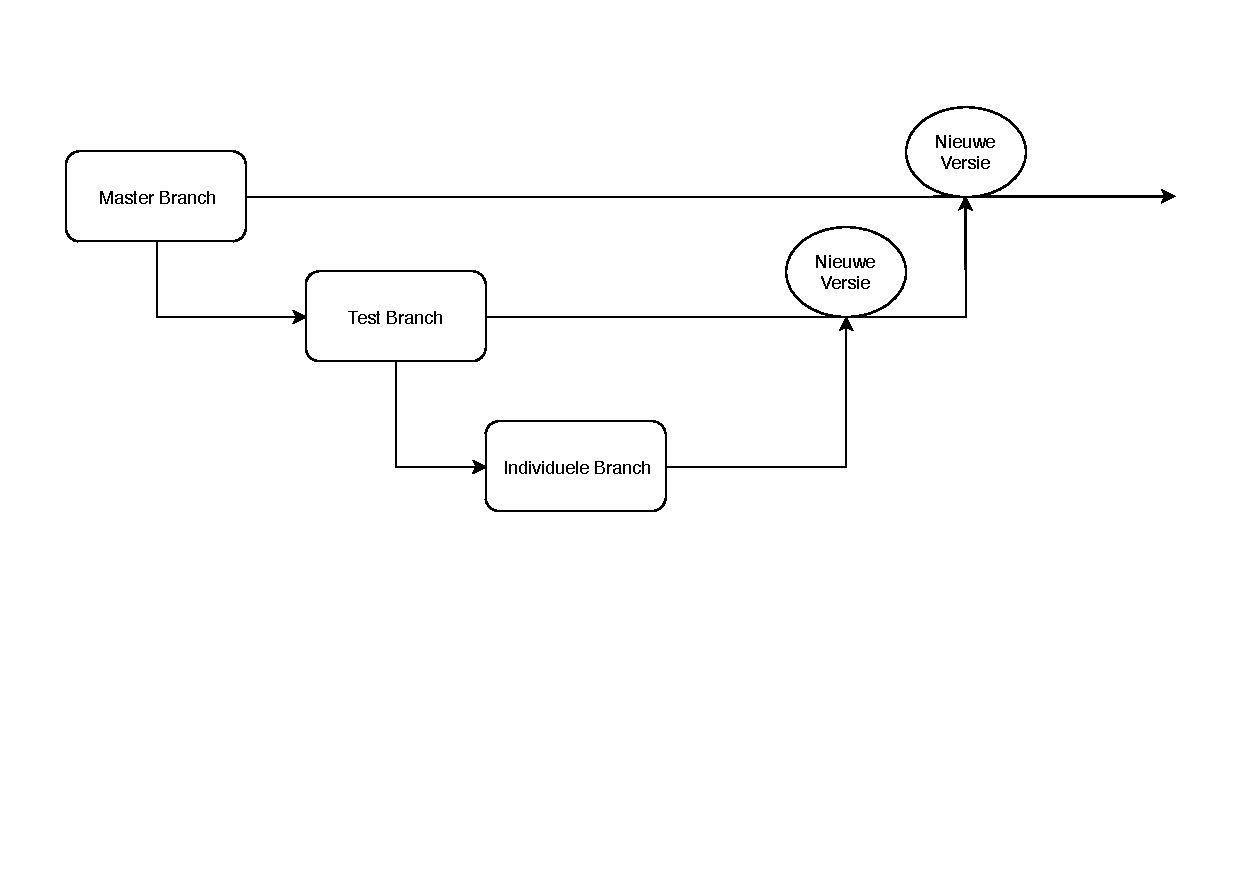
\includegraphics[height=4in]{git.pdf}
        \caption{GIT FlowWork}
        \label{fig: git model}
\end{figure}

\subsection{Issue \& Risico}

\paragraph{Issue Tracking}
Issue Tracking voor dit project wordt op de GIT bijgehouden.
Om de issue tracking voor dit project te bekijken,
ga naar de Git van dit project.
De issues worden bijgehouden om de problemen tijdens de development
te noteren en te behandelen.
Zo kan er ook aan het eind van het project aangegeven worden,
tegen welke problemen het development team op gelopen heeft.
Bij de issues worden er opdrachten toegewezen aan leden van de groep.\\

Link:

\MVAt~\href{https://github.com/Gewad/Project4Bankalicious/issues}{Git issues}

\paragraph{Risico Log}
Het risico log is opgesteld om in het begin aan te geven
welke risico's op ons te wachten staan.
De risicos worden in dit logboek opgeschreven.
Tijdens het bouwen van dit systeem wordt er rekening gehouden met de risico's
om hen te kunnen verkomen in de eindfase van de development.
Het risico log wordt ook op GIT bijgehouden.\\

Links:

\MVAt~\href{https://github.com/Gewad/Project4Bankalicious/blob/test/opdrachten/opdracht_h/opdracht_h_wondel/risicolog.xlsx}{Persoonlijk: Risicolog}

\MVAt~\href{https://github.com/Gewad/Project4Bankalicious/blob/test/opdrachten/opdracht_hj/opdracht_h_teamonderdeel.xlsx}{Team: Risicolog}

\end{document}
